\documentclass[12pt,dvipsnames]{book}

\usepackage{amsmath}
\usepackage{amsfonts}
\usepackage{amssymb}
\usepackage{amsthm}
\usepackage{booktabs}
\usepackage{xcolor}
\usepackage{listings}
\usepackage{graphicx}
\usepackage[left=2.5cm,right=2.5cm,bottom=2cm]{geometry}

\usepackage[colorlinks=true,
	linkcolor=blue, urlcolor=blue,
	pdfauthor={L. Felipe Martins},
	pdfsubject={Computational number theory},
	pdfkeywords={number theory, computations, cryptography},
	pdfstartview=FitH,
	pdfview=FitH]{hyperref}

%\usepackage{enumitem}
%\setlist{nolistsep}

%\usepackage{tikz}
%\usetikzlibrary{arrows, positioning, calc}
%\tikzstyle{vertex}=[draw, fill=green!15, circle, minimum size=20pt, inner sep=0pt]
%
%\newcommand{\ttnot}{\ensuremath{\mathtt{Not}}}
%\newcommand{\ttand}{\ensuremath{\mathtt{And}}}
%\newcommand{\ttor}{\ensuremath{\mathtt{Or}}}
%\newcommand{\ttimp}{\ensuremath{\mathtt{Imp}}}
%\newcommand{\tteqv}{\ensuremath{\mathtt{Eqv}}}
%\newcommand{\opnot}{\ensuremath{\neg}}
%\newcommand{\opand}{\ensuremath{\land}}
%\newcommand{\opor}{\ensuremath{\lor}}
%\newcommand{\opimp}{\ensuremath{\rightarrow}}
%\newcommand{\opeqv}{\ensuremath{\leftrightarrow}}
%\newcommand\Z{\ensuremath{\mathbb{Z}}}
%\newcommand\N{\ensuremath{\mathbb{N}}}
%\newcommand\R{\ensuremath{\mathbb{R}}}
%\newcommand\Q{\ensuremath{\mathbb{Q}}}
%\newcommand\C{\ensuremath{\mathbb{C}}}
%\newcommand{\kw}[1]{$\mathtt{#1}$}
%\newcommand{\interp}[1]{\ensuremath{{\cal #1}}}

\theoremstyle{plain}
\newtheorem{theorem}{Theorem}[section]
\newtheorem{proposition}[theorem]{Proposition}
\newtheorem{lemma}[theorem]{Lemma}
\newtheorem{corollary}[theorem]{Corollary}
\newtheorem{conjecture}[theorem]{Conjecture}
\newtheorem*{conjecture*}{Conjecture}
\newtheorem{criterion}[theorem]{Criterion}
\newtheorem{principle}[theorem]{Principle}
\newtheorem{property}[theorem]{Property}

\theoremstyle{definition}
\newtheorem{definition}[theorem]{Definition}
\newtheorem{condition}[theorem]{Condition}
\newtheorem{example}[theorem]{Example}
\newtheorem{exercise}{}[section]
\newtheorem*{solution}{\emph{\textbf{Solution}}}

\theoremstyle{remark}
\newtheorem{remark}[theorem]{Remark}
\newtheorem{note}[theorem]{Note}
\newtheorem{notation}[theorem]{Notation}
\newtheorem{claim}[theorem]{Claim}


\begin{document}

\lstset{
	language=Python,
	basicstyle=\small\ttfamily,
	keywordstyle=\ttfamily\color{NavyBlue},
	identifierstyle=\ttfamily\color{Black},
	commentstyle=\ttfamily\color{Gray},
	stringstyle=\ttfamily\color{Green},
	showstringspaces=false,
	numbers=left, numberstyle=\tiny, numbersep=5pt,
%	moredelim=[s][\ttfamily\color{Black}]{ghci}{>},
	moredelim=[is][\itshape\sffamily\color{OliveGreen}]{>>}{<<},
%	moredelim=[is][\ttfamily\color{Black}]{||>}{<||}
}

%!TEX root = ode-systems.tex
\chapter{Computing Solutions of a System of ODEs}

Systems of differential equations come up because nature is complex. Most systems of interest in science and engineering are made of many interacting components with multiple relationships. Each component must be represented by a variable and, in the context of differential equation, each has to be modeled by a separate equation.

In this chapter, the reader will:

\begin{itemize}
\item Learn about the predator-prey model, an important application of differential equations to the study of an ecological system.
\item Learn how to load the Python libraries necessary to solve systems of differential equations.
\item Explore the use of the \texttt{odeint} function, which is the main tool we will use to solve systems of differential equations.
\item Learn how to produce different graphical displays of solutions of a system of differential equations.
\end{itemize}

The exercises at the end of the chapter present several other examples and give the reader an idea of the breadth of application areas that can be studied with systems of differential equations.

\section{The Predator-Prey Model}

This model describes two animal species in the wild, traditionally referred to as ``rabbits'' and ``foxes''. The following assumptions are made about the two populations and their interactions:

\begin{itemize}
\item Without the presence of foxes, the rabbit population will grow exponentially without limit. This, of course, is a simplification, since in a real population there would be environmental limits to growth.
\item Without the presence of rabbits, the fox population will decay exponentially and become extinct. This is tacitly assuming that foxes prey exclusively on rabbits. Most predators will hunt more than one prey species.
\item The effect of predation on the growth of each species is proportional to the product of the sizes of the rabbit and fox populations. This is also  a simplification, since it essentially posits that, the capacity for hunting of the fox population is unlimited. Typically, there is a saturation point after which, no matter how large the rabbit population is, the level of predation remains constant.
\end{itemize}

Denoting by $R(t)$ and $F(t)$, respectively, the sizes of the rabbit and fox populations, the assumptions above entail the following model:
\begin{align}
\label{rabbit-eq}R'&=aR-bRF\\
\label{fox-eq}F'&=-cF+dRF
\end{align}
The parameters $a$, $b$, $c$ and $d$ are assumed to be positive, and can be interpreted as follows:
\begin{itemize}
\item $a$ is the per-capita growth rate of the rabbit population in the absence of foxes.
\item $b$ represents the effect of predation on the rabbit population.
\item $c$ is the per-capita decay rate of the fox population in the absence of rabbits.
\item $d$ represents the effect of predation on the fox population.
\end{itemize}
The equations in~\eqref{rabbit-eq},~\eqref{fox-eq} can be solved analytically to provide an implicit relationship between the variables $R$ and $F$ (see Exercise~\ref{ex-rabbit-fox-implicit}). In the next sections we will describe, instead, an experimental approach, based on numerical simulations.

\section{Computing Solutions}

We now concentrate on the task of computing solutions for the predator-prey systems. The computations presented here use numerical methods and are, thus, approximations to the actual solutions. The details of the computation (including choice of step sizes and accuracy) are hidden from the user. This suits us well right now, and readers interested in the details of the computations are referred to the documentation of the \texttt{odeint} method
\footnote{\url{http://docs.scipy.org/doc/scipy/reference/generated/scipy.integrate.odeint.html\#scipy.integrate.odeint}}.

The following code assumes that the reader has an open Jupyter notebook, and that a standard distribution, such as Anaconda, has been installed. To solve a system of differential equations, the first step is to load the required libraries into the Jupyter workspace, which can be done by executing a code cell with the statements shown below:
\begin{lstlisting}
%matplotlib inline
import numpy as np
import matplotlib.pyplot as plt
from scipy.integrate import odeint
\end{lstlisting}
The code displayed above achieves the following:
\begin{itemize}
\item \textbf{Line 1}: Sets up the graphics library \texttt{matplotlib} so that graphs as displayed inline. This means that each graph appears right after the computing cell that creates it.
\item \textbf{Line 2}: Import the module \textbf{numpy} with the alias \textbf{np}. \textbf{numpy} is the module that defines the \textbf{array} object, which is a Python data structure optimized for computational mathematics.
\item \textbf{Line 3}: Import the module \textbf{matplotlib.pyplot} with the alias \textbf{plt}. \textbf{pyplot} is a collection of objects and functions for interactive graphics.
\item \textbf{Line 4}: Import the \textbf{odeint} function from the module \textbf{scipy.integrate}. \textbf{odeint} is the solver for systems of differential equations that we will be using.
\end{itemize}

The code shown above needs to be run only once for the entire notebook. So, it is typical to put it on a cell right on top of the notebook.

The next task is to define of the system of differential equations~\eqref{rabbit-eq},~\eqref{fox-eq} in Python. The interface of the function \textbf{odeint} requires this to be done with a function with a specific signature. In our situation, we can use the code below, which should be run in a separate computing cell:
\begin{lstlisting}
def pred_prey_system(x, t, *args):
    a, b, c, d = args
    R, F = x
    return np.array([a*R - b*R*F, -c*F + d*R*F])
\end{lstlisting}
These code lines do the following:
\begin{itemize}
\item \textbf{Line 1:} This starts the definition the Python function \texttt{pred\_prey\_system}. The input arguments are:
	\begin{itemize}
	\item \texttt{x} is a 2-component \texttt{numpy} array, representing the $(R, F)$ pair of variables.
	\item \texttt{t} is a floating point value, representing time.
	\item \texttt{*args} is a tuple of extra arguments, used, in our example, to pass the parameters $a$, $b$, $c$ and $d$. The \texttt{*} notation is a Python feature that allows the tuple to be passed without enclosing parenthesis. 
	\end{itemize}
\item \textbf{Line 2:} Unwrap \texttt{args} and store its values in the variables \texttt{a}, \texttt{b},\texttt{c} and \texttt{d}.
\item \textbf{Line 3:} Unwrap \texttt{x} and store its values in the variables \texttt{R} and \texttt{F}.
\item \textbf{Line 4:} Return the array that represents the right-hand side of equations in the system~\eqref{rabbit-eq},~\eqref{fox-eq} evaluated at the current values of $R$, $F$ and $t$.
\end{itemize}
Once we have defined the system, we can compute solutions as indicated below:
\begin{lstlisting}
a, b, c, d = 0.75, .2, 1.15, .1
tvalues = np.linspace(0, 10, 11)
init = [15, 20]
solution = odeint(pred_prey_system, init, tvalues, args=(a,b,c,d))
\end{lstlisting}
Notice that running this cell will not produce any output, since the result of the computation is stored in the variable \texttt{solution}. The code above solves the predator-prey system for the parameter values $a=0.75$, $b=0.2$, $c=1.15$, $d=0.1$ and the initial conditions $R(0)=15$, $P(0)=20$. The details of the computation are as follows:
\begin{itemize}
\item \textbf{Line 1:} Set the parameter values \texttt{a}, \texttt{b}, \texttt{c} and \texttt{d}. 
\item \textbf{Line 2:} Define the array \texttt{tvalues}. The expression \texttt{np.linspace(0, 10, 11)} generates 11 equally spaced points in the interval $[0,10]$. Notice that both endpoints are included in the generated array.
\item \textbf{Line 3:} Define the list \texttt{init}, which contains the initial values of the populations.
\item \textbf{Line 4:} Call \texttt{odeint} to compute the solution and store the output in the array \texttt{solution}. The arguments to the call are:
	\begin{itemize}
	\item \texttt{pred\_prey\_system} is the function that specifies the system of differential equations, as defined in the previous computation cell.
	\item \texttt{init} is an array containing the initial condition.
	\item \texttt{tvalues} is an array that specifies the times at which the solution is be computed. The first value, \texttt{tvalues[0]}, is the time at which the initial condition is given.
	\item  \texttt{args=(a,b,c,d)} sets the parameter values for this instance of the model.
	\end{itemize}
\end{itemize}
We can see the results of the computation by entering the variable name \texttt{solutions} by itself in a computation cell:
\begin{lstlisting}
solution
\end{lstlisting}
This produces the output:
\begin{lstlisting}
array([[ 15.        ,  20.        ],
       [  1.28022691,  10.17471157],
       [  0.76907897,   3.5250347 ],
       [  1.05575964,   1.21782139],
       [  1.91904005,   0.44474622],
       [  3.83220224,   0.18548621],
       [  7.89563598,   0.10296241],
       [ 16.39501079,   0.10433694],
       [ 33.47233713,   0.36492363],
       [ 43.63108633,   8.70404658],
       [  2.98858554,  15.85969476]])
\end{lstlisting}
The solution is provided in a 2-dimensional array, with the rabbit population in the first column and the fox population in the second column. Notice that the values of the time variable are not included in the solution, since they are available in the \texttt{tvalues} array.

\section{Generating Solution Plots}

Producing solution plots is one of the most important steps in the study of a a system of differential equations. Let's first consider the problem of generating a solution for a larger set of time values, as indicated in the following code:
\begin{lstlisting}
a, b, c, d = 0.75, .2, 1.15, .1
tvalues = np.linspace(0, 30, 600)
init = [15, 20]
solution = odeint(pred_prey_system, init, tvalues, args=(a,b,c,d))
\end{lstlisting}
This code is very similar to the previous computation, the only difference being on the line defining \texttt{tvalues}, where we set the maximum time to 60 and the number of time values to 600.

In order to plot the solutions, it is convenient to have the vectors representing the rabbit and fox populations in separate arrays. This can be done with the line of code below:
\begin{lstlisting}
Rvalues, Fvalues = solution.transpose()
\end{lstlisting}
This code first transposes the \texttt{solution} array, so that the two populations are across the rows of the array. The rows of the array are then assigned to the variables \texttt{Rvalues} and \texttt{Fvalues}, which will be used to produce the plots.

To create a time-dependent plot of the solutions we can use the following code:
\begin{lstlisting}
plt.plot(tvalues, Rvalues, color='green', lw=2)
plt.plot(tvalues, Fvalues, color='red', lw=2)
plt.title('Predator-prey model ' + 
    'a={:3.2f}, b={:3.2f}, c={:3.2f}, d={:3.2f}'.format(a,b,c,d))
plt.xlabel('$t$')
plt.ylabel('$R(t),F(t)$')
plt.legend(['$R(t)$','$F(t)$'], loc='upper left')
None
\end{lstlisting}
This will produce the plot shown in Figure~\ref{fig-predprey-timedep}.
The plot is generated with several successive calls to functions in the module \texttt{plt}. Each call adds a component to the graph. This is called the ``state machine'' approach to construct a graph, which is convenient to produce graphs in an interactive fashion. The purpose of each call is discussed below:
\begin{itemize}
\item \textbf{Lines 1 and 2:} Generate the graphs of the functions $R(t)$ and $F(t)$. In each call, the data is given in two arrays, which are the values plotted, respectively, across the horizontal and vertical axes. The remaining arguments to \texttt{plot} specify the color and line width of each graph.
\item \textbf{Lines 3 and 4:} Create the title for the plot. The title is given as a formatted string, and reports the values of the parameters $a$, $b$, $c$ and $d$. For purposes of display on the book page, the string was split in two pieces, but might as well be typed in a single line.
\item \textbf{Lines 5 and 6:} Print the axes labels. Notice the use of \TeX{}, which is a feature available in most \texttt{matplotlib} functions.
\item \textbf{Line 7:} Add a legend to the plot, placing it on the upper-left corner, so that it does not interfere with the plot.
\item \textbf{Line 8:} The default behavior in an executed cell is to print the last computed value. The output of the functions in the \texttt{plt} module is irrelevant to us, and adding \texttt{None} at the end of the cell prevents its output.
\end{itemize}

\begin{figure}[h]
\caption{Time-dependent plot of a solution to the predator-prey model.}
\label{fig-predprey-timedep}
\begin{center}
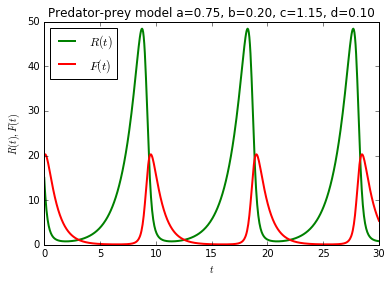
\includegraphics[scale=0.6]{predprey-timedep.png}
\end{center}
\end{figure}

Notice the apparent periodic behavior of the solution. This cyclical interplay in the population dynamics is typical of predator-prey interactions in the wild, although the data will never be as regular as the solutions of the differential equations. The periodical behavior of the solutions is even more evident in the phase diagram of the solution, which can be produced with the code below:
\begin{lstlisting}
plt.plot(Rvalues, Fvalues, lw=2)
plt.title('Predator-prey model ' + 
    'a={:3.2f}, b={:3.2f}, c={:3.2f}, d={:3.2f}'.format(a,b,c,d))
plt.xlabel('$R$')
plt.ylabel('$F$')
None
\end{lstlisting}
The graph produced is displayed in Figure~\ref{fig-predprey-phase1}. The code is very similar to the previous example, the main difference being that now, in Line 1, we plot \texttt{Rvalues} in the horizontal axis and \texttt{Fvalues} in the vertical axis. Also notice that we omit the legend, since the meaning of the curve is clear from the axis labels.

\begin{figure}[h]
\caption{Phase plot of a solution to the predator-prey model.}
\label{fig-predprey-phase1}
\begin{center}
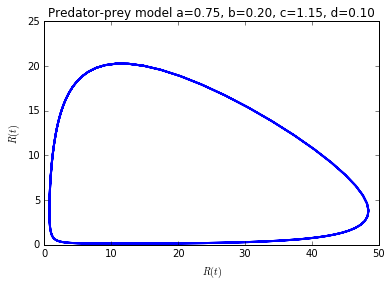
\includegraphics[scale=0.6]{predprey-phase1}
\end{center}
\end{figure}

The closed curve representing the solution makes the periodicity of the solution evident. Phase plots have the advantage that solutions for several different initial conditions can be plotted simultaneously. This is illustrated by the following code:
\begin{lstlisting}
a, b, c, d = 0.75, .2, 1.15, .1
tvalues = np.linspace(0, 15, 600)
inits = [[15, 20], [15, 10], [15, 30],
         [15, 15], [15, 25]]
for init in inits:
    solution = odeint(pred_prey_system, init, tvalues, args=(a,b,c,d))
    Rvalues, Fvalues = solution.transpose()
    plt.plot(Rvalues, Fvalues, lw=2, color='blue')
plt.title('Predator-prey model ' + 
    'a={:3.2f}, b={:3.2f}, c={:3.2f}, d={:3.2f}'.format(a,b,c,d))
plt.xlabel('$R(t)$')
plt.ylabel('$R(t)$')
None
\end{lstlisting}
Please refer to Figure~\ref{fig-predprey-phase2}. The code shown above is mostly a rearrangement of code seen before. The main differences are discussed below:
\begin{itemize}
\item \textbf{Lines 3, 4:} Since we want to plot solutions for several different initial conditions, we define a Python list called \texttt{inits} containing all the initial conditions we want to consider.
\item \textbf{Lines 5--8:} The computation and plotting of each solution are now wrapped into a \texttt{for} loop. The \texttt{for} control structure, specified in line 5, will step over the elements of the list \texttt{inits}, assigning each of the initial conditions to the variable \texttt{init} in succession. For each initial condition, we compute the solution and then plot it in the body of the loop.
\end{itemize}

\begin{figure}[h]
\caption{Phase plot of several solutions to the predator-prey model.}
\label{fig-predprey-phase2}
\begin{center}
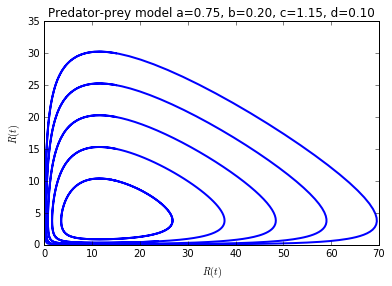
\includegraphics[scale=0.6]{predprey-phase2}
\end{center}
\end{figure}

It becomes evident that all solutions plotted are periodical. In the exercises, the reader is invited to explore the nature of the solutions in more detail.

\section{Conclusions}

In this chapter, the reader learned the following:
\begin{itemize}
\item How to represent the interaction of two species in a predator-prey situation.
\item How to load the Python modules necessary to solve a system of differential equations.
\item How to define a function, \texttt{pred\_prey\_system} that represents the system of differential equations.
\item How to use the function \texttt{odeint} to solve the system, and how to access the solution.
\item How to produce several different types of displays representing solutions using module \texttt{matplotlib.pyplot} (referred to as \texttt{plt} in the code).
\end{itemize}

In the next chapter we will concentrate on linear systems, and how to specialize the methods of this chapter to that important particular case.

\section{Exercises}

\begin{exercise} 
\label{ex-rabbit-fox-implicit}
Equations~\eqref{rabbit-eq},~\eqref{fox-eq} can be written using Leibniz notation for derivatives as follows:
\begin{align}
\label{rabbit-eq1}\frac{dR}{dt}&=aR-bRF\\
\label{fox-eq1}\frac{dF}{dt}&=-cF+dRF
\end{align}
This suggests dividing equation~\eqref{rabbit-eq1} by equation~\eqref{fox-eq1} to obtain:
\begin{equation}
\label{rabbit-fox-eq}
\frac{dR}{dF}=\frac{aR-bRF}{-cF+dRF}
\end{equation}
\begin{enumerate}
\item Use separation of variables on equation~\ref{rabbit-fox-eq} to obtain an implicit formula relating the variables $R$ and $F$.
\item Visit the matplotlib website (\url{http://matplotlib.org}) and search the documentation for a function that plots implicitly defined equations, and use it to draw a plot of $R$ versus $F$, using the equation from the previous item.
\end{enumerate}
\end{exercise}

\begin{exercise} The version of the predator-prey model described in this chapter makes the unrealistic assumption that the rabbit population can grow without limit. A more reasonable assumption is that, in the absence of predators, the rabbit population grows according to a \emph{logistic model}:
\[
R'=aR\left(1-\frac{R}{N}\right)
\]
The parameter $N$ is a positive constant called the \emph{carrying capacity}.
\begin{enumerate}
\item Modify the system~\eqref{rabbit-eq},~\eqref{fox-eq} to represent this assumption.
\item Conduct a graphical analysis of the system, by plotting solutions to various different sets of parameters and initial conditions. Describe qualitatively the solutions and interpret them in terms of a predator-prey situation.
\item Do you think, in this case, it is possible to find an implicit relationship between $R$ and $F$, as was done in Exercise~\ref{ex-rabbit-fox-implicit}? Explain why or why not.
\end{enumerate}
\end{exercise}

\begin{exercise} The \emph{Van der Pol} oscillator is used to describe the dynamics of a certain electronic component, and is described by the system of differential equations:
\begin{align*}
x' &= y\\
y' &= \mu(1-x^2)y-x
\end{align*}
where the parameter $\mu$ is positive. Conduct a series of numerical experiments to investigate solutions of this system for different values of $\mu$. Then, describe the dynamics of the solutions.  
\end{exercise}

\begin{exercise}
The \emph{SIR model} for spread of an infection classifies individuals in the infected population in three \emph{compartments}:
\begin{itemize}
\item $S(t)$ represents the number of individuals that are \emph{susceptible} to be infected at time $t$.
\item $I(t)$ represents the number of individuals that are \emph{infected} at time $t$.
\item $R(t)$ represents the number of individuals that are \emph{removed} from the population, either because they acquired immunity after infection, or due to death.
\end{itemize}
Assuming that the population is fixed:
\begin{equation}
\label{eq-SIR-N}
N=S(t)+I(t)+R(t)
\end{equation}
the following system of differential equations can be used to describe the evolution of the infection:
\begin{align}
\label{eq-SIR-S}
S' &= -\frac{\beta SI}{N}\\
\label{eq-SIR-I}
I' &= \frac{\beta SI}{N}-\gamma I\\
\label{eq-SIR-R}
R' &= \gamma I
\end{align}
\begin{enumerate}
\item By taking the derivative in equation~\ref{eq-SIR-N} we get $S'(t)+I'(t)+R'(t)=0$. Show that this is compatible with equations~\ref{eq-SIR-S}--\ref{eq-SIR-R}.
\item Using equation~\ref{eq-SIR-N}, derive a system of differential equations that involves only the variables $I$ and $R$.
\item Conduct numerical experiments to investigate the dynamics of the epidemics for several different parameter values. Of special interest is to determine for which parameter values will the infection take hold and eventually infect the whole population, and for which values the infection will eventually subside.
\end{enumerate}
\end{exercise}
































%\input{ch02.tex}

\end{document}

















































